\chapter{Diseño e Implementación de la Infraestructura}
\label{chap:diseno_implementacion}

El capítulo documenta el diseño y la implementación de la solución de firma electrónica: la infraestructura base, la validación del contenedor LXC y la PaaS Coolify, los servicios contenerizados que integran la plataforma, su vinculación con PostgreSQL y MinIO dentro de la red institucional, y la integración con Google OAuth 2.0 y el \textit{relay} SMTP de Brevo.

\section{Topología de Red y Arquitectura General}
\label{sec:topologia_arquitectura}

La topología del sistema se organizó en capas para preservar el aislamiento entre componentes, controlar la exposición de servicios y sostener la disponibilidad operativa. En este esquema, el tráfico proveniente de Internet (nivel WAN) ingresa a la red de área local de la facultad (nivel LAN), donde se ubican los contenedores de Docker, entre ellos Documenso y PostgreSQL.

La Figura \ref{fig:arquitectura_global} resume el recorrido de una petición web externa a través de tres niveles:

\begin{enumerate}
    \item Capa de Borde (\textit{Reverse Proxy} Nginx): las peticiones dirigidas al dominio institucional \nolinkurl{documentos.facet.unt.edu.ar} son recibidas inicialmente por el \textit{reverse proxy} perimetral Nginx de la facultad. Este componente gestiona la terminación SSL mediante certificados de Let's Encrypt y reenvía el tráfico HTTP/HTTPS hacia la red interna, tal como puede apreciarse en las Figuras~\ref{fig:headers_nginx} y \ref{fig:certificado_tls}.
    \item Capa PaaS (Coolify): el tráfico es dirigido a un contenedor Linux (LXC) dentro del hipervisor Proxmox VE. En esta capa opera la PaaS Coolify, que gestiona una instancia interna de Traefik que enruta dinámicamente las peticiones hacia el servicio correspondiente.
    \item Capa de Servicios (Contenedores Docker): finalmente, la solicitud llega al contenedor de la aplicación Documenso. Este se comunica de forma interna (mediante redes privadas de Docker) con su base de datos PostgreSQL y el servicio contenerizado Browserless, y a través de la red local con el servidor de almacenamiento TrueNAS/MinIO.
\end{enumerate}

En este esquema, ni la dirección IP del servidor ni los puertos internos de Docker quedan expuestos directamente a Internet. Todo el flujo de datos atraviesa el \textit{reverse proxy} perimetral de la facultad, que actúa como único intermediario entre los usuarios externos y la red local.

\begin{figure}[!htbp]
    \centering
    \includegraphics[width=0.9\textwidth]{figuras/capitulo3/TopologiadeRedyArquitecturaGeneral.png}
    \caption[Arquitectura Global del Sistema]{Diagrama de flujo de tráfico y arquitectura de capas del sistema de firma electrónica.}
    \label{fig:arquitectura_global}
\end{figure}

\begin{figure}[!htbp]
    \centering
    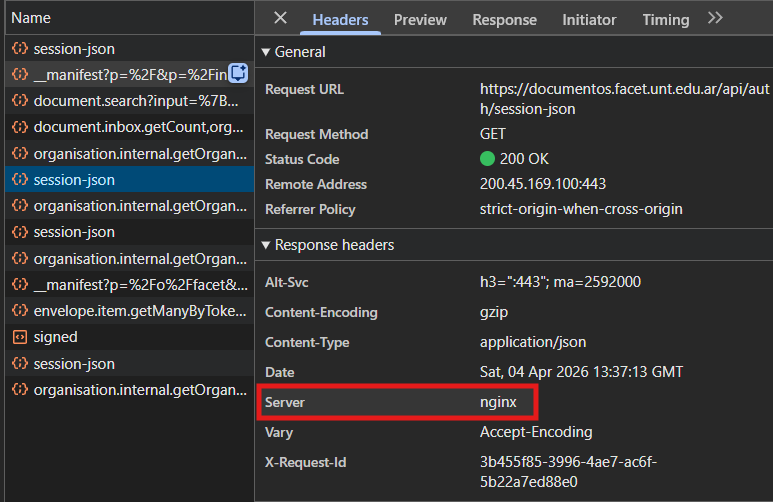
\includegraphics[width=0.95\textwidth]{figuras/capitulo3/headers_https_documenso-server_ngnix.png}
    \caption[Cabeceras HTTP del dominio institucional]{Cabeceras HTTP de la respuesta del dominio institucional, con \texttt{Server: nginx}.}
    \label{fig:headers_nginx}
\end{figure}

\begin{figure}[!t]
    \centering
    {\setlength{\fboxsep}{3pt}\colorbox{black}{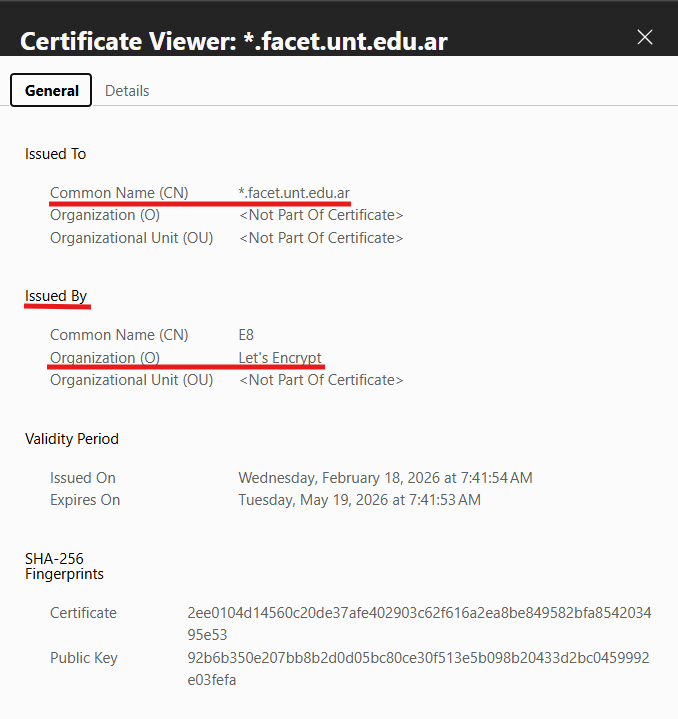
\includegraphics[width=0.52\textwidth]{figuras/capitulo3/certificadoTLS.png}}}
    \caption[Certificado TLS del dominio institucional]{Certificado TLS presentado por el dominio institucional, emitido para \texttt{*.facet.unt.edu.ar} por Let's Encrypt.}
    \label{fig:certificado_tls}
\end{figure}

\FloatBarrier

\section{Infraestructura Base y Entorno PaaS}
\label{sec:infraestructura_base}

La implementación no partió de un despliegue desde cero, sino de una infraestructura base previamente aprovisionada por el área de sistemas de la FACET. En esta etapa, el trabajo consistió en auditar ese entorno, comprobar que resultara suficiente y usarlo como base para desplegar Documenso sobre la PaaS ya disponible.

\subsection{Auditoría del Entorno LXC y Configuración Base}

La etapa de despliegue comenzó con la auditoría técnica de un contenedor LXC con Ubuntu 22.04 LTS, aprovisionado por la facultad sobre el hipervisor Proxmox VE. El contenedor disponía de 8~núcleos lógicos, 8~GB de memoria RAM, un disco raíz de 50~GB y un volumen de montaje adicional de 160~GB, recursos que superan holgadamente los requerimientos combinados de Coolify \cite{coolify_reqs} y Documenso \cite{documenso_reqs} (4~vCPUs, 4~GB de RAM y 50~GB de almacenamiento en conjunto).

El entorno se configuró como un contenedor no privilegiado para aislar los procesos del nivel de ejecución del servidor físico y mitigar el impacto ante un incidente de seguridad. A su vez, se habilitó el anidamiento (\texttt{nesting=1}), requisito para que el motor de Docker instancie redes y orqueste sus propios subcontenedores dentro del LXC.

\subsection{Justificación del Uso de Coolify como PaaS}

Inicialmente, se evaluó desplegar Documenso sobre una máquina virtual (VM) o un contenedor LXC dedicados en Proxmox. Esa alternativa se descartó porque implicaba montar y mantener manualmente toda la infraestructura asociada: un \textit{reverse proxy} adicional para publicar la aplicación, el enrutamiento hacia los servicios auxiliares y el despliegue separado de PostgreSQL, Browserless y el \textit{proxy} hacia MinIO. En cambio, se aprovechó la instancia de Coolify ya disponible en la infraestructura. Esto permitió centralizar la operación sin incorporar una nueva VM ni sobredimensionar recursos.

En la práctica, la PaaS resolvió tareas que, en un despliegue manual, hubieran incrementado la carga operativa y el margen de error:

\begin{itemize}
    \item Gestión de red: enrutamiento interno dinámico mediante Traefik, que recibe el tráfico del \textit{reverse proxy} perimetral y lo dirige al puerto correspondiente de cada contenedor.
    \item Aislamiento: segmentación de servicios en redes virtuales de Docker para mantener separados los componentes.
    \item Mantenimiento: interfaz centralizada para inyectar variables de entorno, gestionar volúmenes y consultar logs en tiempo real.
    \item Respaldo: integración con almacenamiento S3 compatible, utilizada más adelante para automatizar los respaldos de PostgreSQL sobre MinIO.
\end{itemize}

En esta arquitectura conviene diferenciar el rol de cada capa. Proxmox VE corre sobre el servidor físico, cuya IP en la LAN es \texttt{192.168.80.39}. Su función consiste en asignar recursos de cómputo, memoria y almacenamiento a los contenedores y máquinas virtuales que administra. El hipervisor no participa del enrutamiento ni del procesamiento del tráfico HTTP/HTTPS de las aplicaciones.

El contenedor LXC, en cambio, se conecta a la LAN de la facultad mediante un puente virtual (bridge) configurado en Proxmox y obtiene su propia IP, \texttt{192.168.80.65}, como un nodo independiente de la red local. Para Docker y Traefik, ese LXC actúa como sistema anfitrión: allí se publican los puertos \texttt{80} y \texttt{443} y desde allí se resuelve el enrutamiento interno hacia los contenedores. Así, Proxmox queda en el plano de gestión de la infraestructura, mientras que el LXC concentra el plano de datos de la aplicación.

La Figura \ref{fig:zoom_coolify} muestra esta arquitectura anidada y el modo en que Coolify gestiona el enrutamiento interno mediante Traefik, manteniendo a Documenso separado de otros servicios desplegados sobre ese LXC.

\begin{figure}[H]
    \centering
    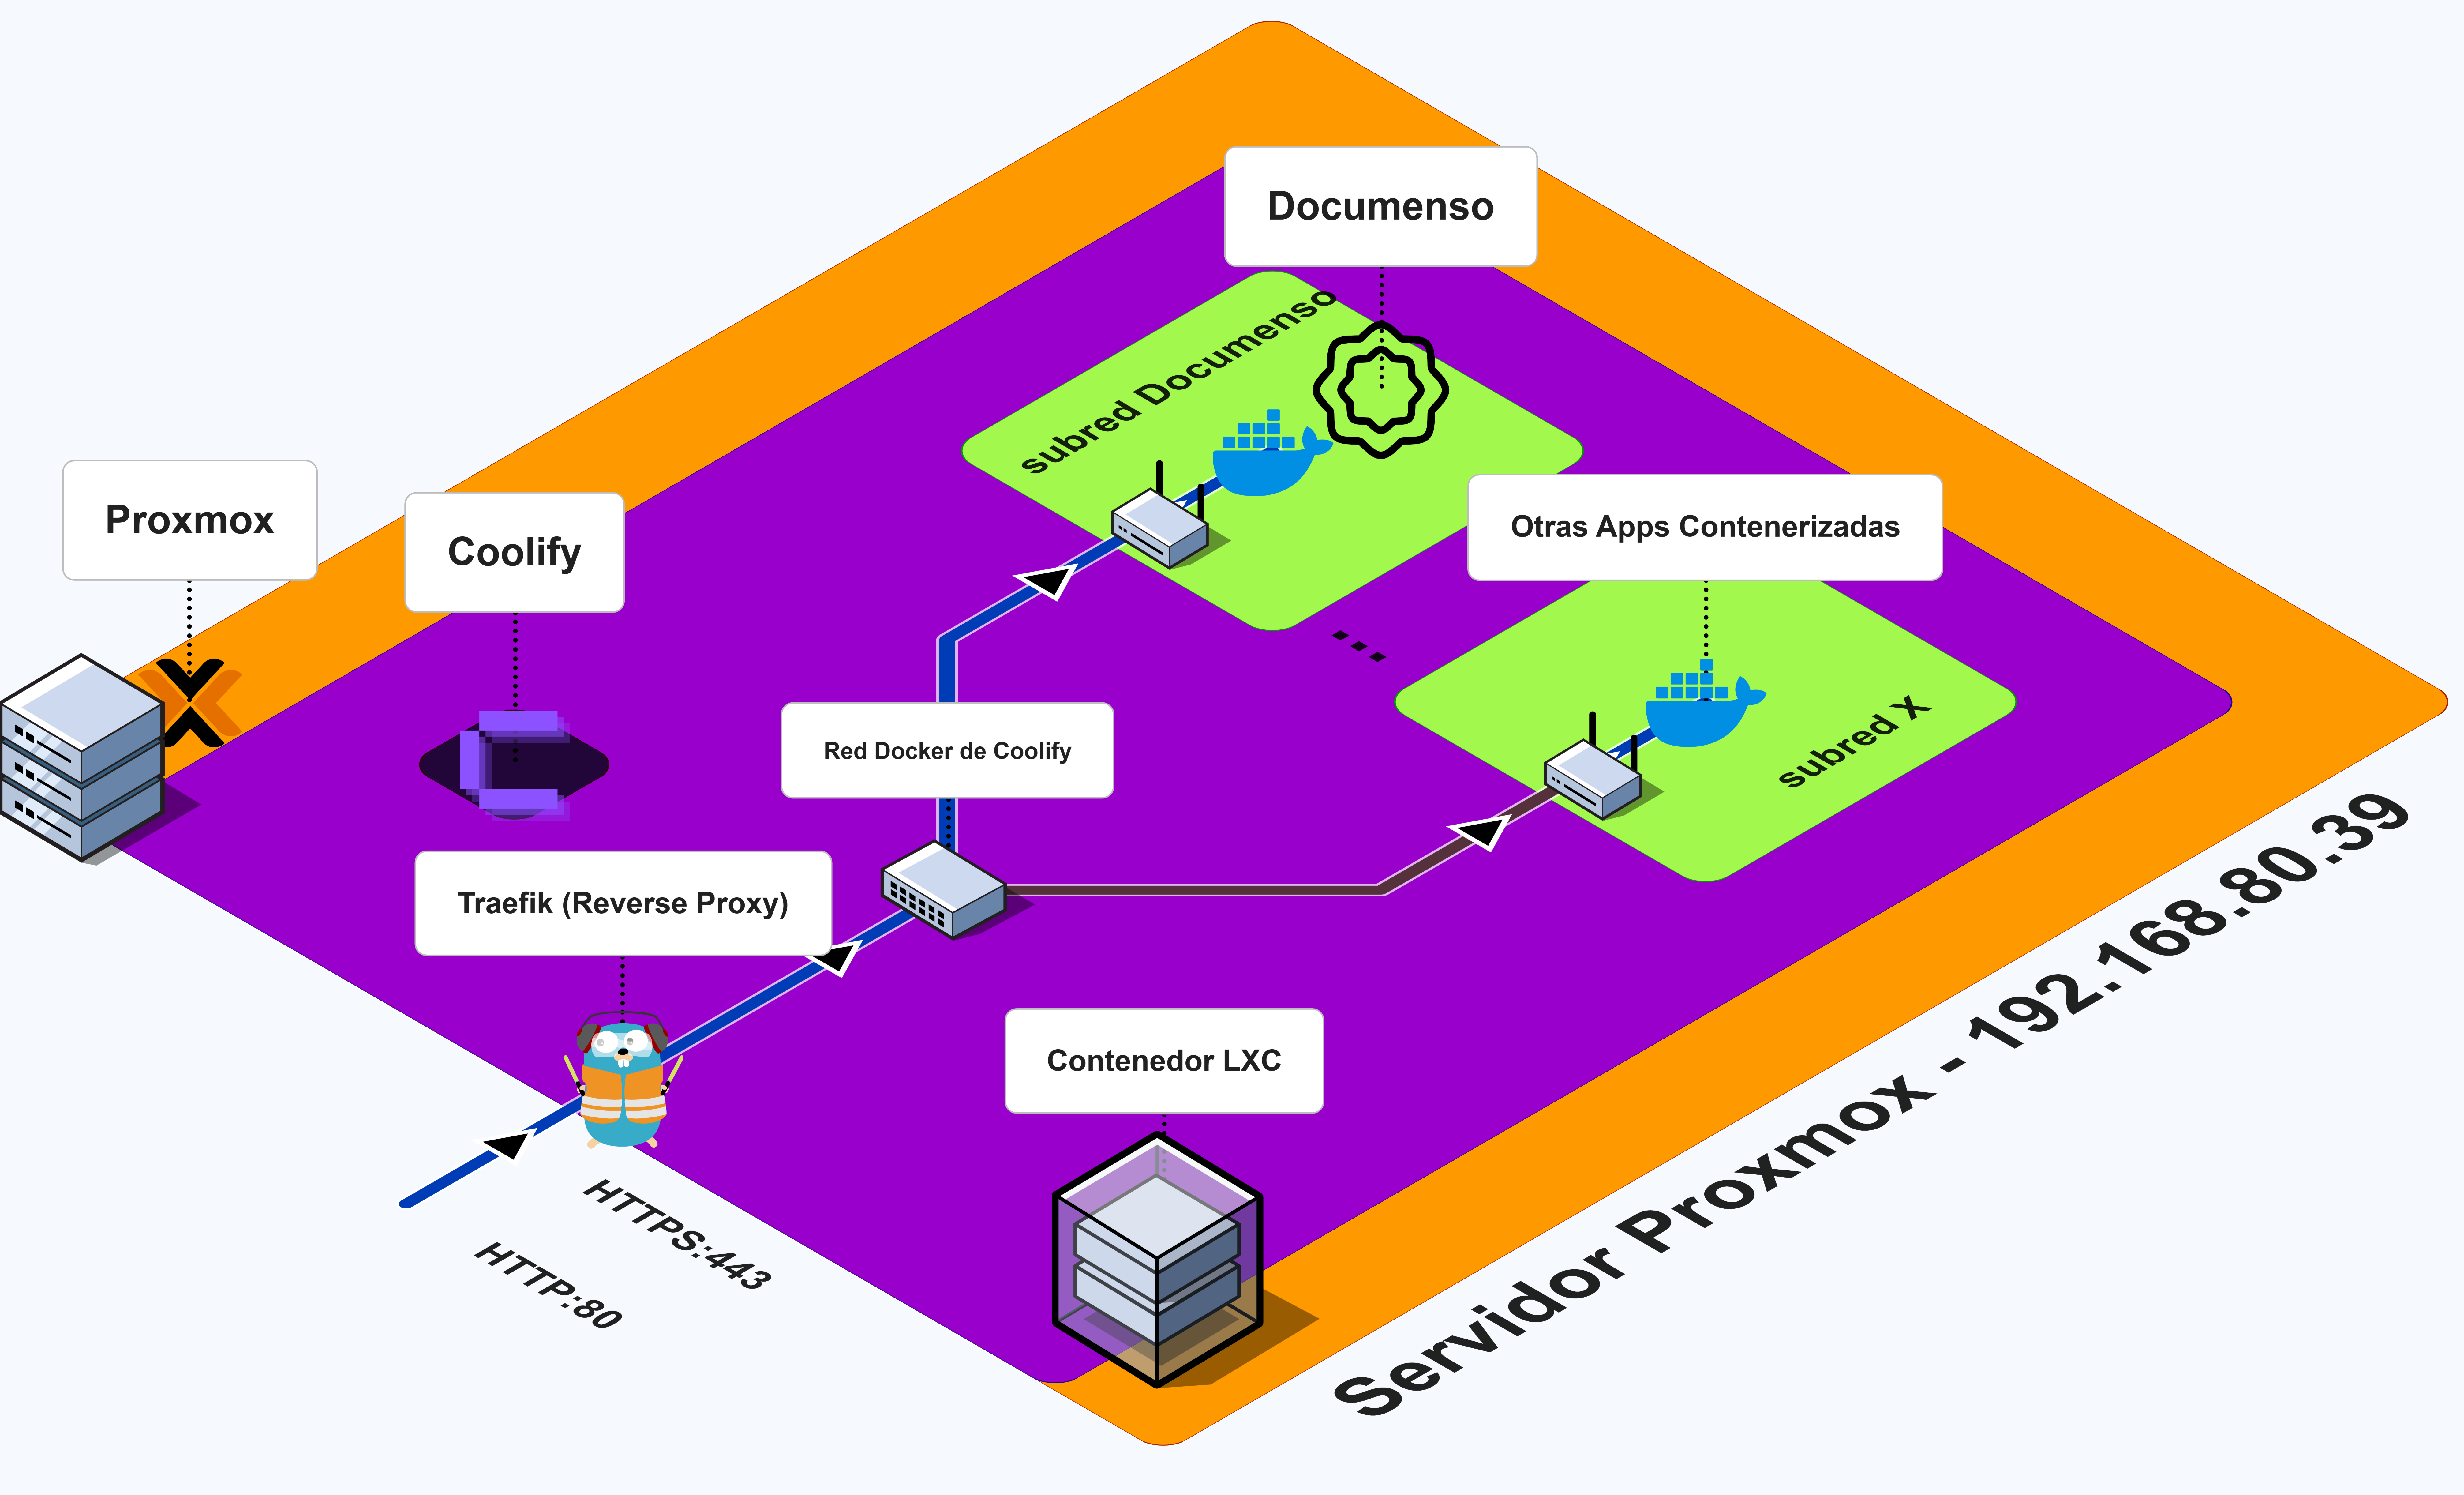
\includegraphics[width=0.9\textwidth]{figuras/capitulo3/ZoomProxmoxCoolify.png}
    \caption[Topología interna de la PaaS Coolify]{Arquitectura anidada y segmentación de redes virtuales Docker dentro del contenedor LXC base.}
    \label{fig:zoom_coolify}
\end{figure}

\section{Configuración de Servicios y Despliegue de Documenso}
\label{sec:configuracion_servicios}

Una vez validada la capa base, el trabajo avanzó hacia el despliegue de Documenso y sus servicios auxiliares. Para definir esta implementación se tomaron como punto de partida dos referencias: la plantilla oficial de Coolify para Documenso \cite{coolify_documenso_template} y la guía de despliegue con Docker Compose publicada en la documentación de Documenso \cite{documenso_docker_compose_docs}. Ninguna de las dos resolvía por sí sola las necesidades del entorno institucional. A medida que avanzaron las pruebas aparecieron requisitos y problemas no cubiertos inicialmente, lo que obligó a investigar ajustes adicionales e incorporar servicios complementarios. La configuración final surgió de esa combinación entre referencias previas y decisiones tomadas durante la fase de prueba, que se describen en las subsecciones siguientes.

La arquitectura resultante quedó organizada en cuatro servicios contenerizados: PostgreSQL para la persistencia transaccional, Browserless como motor de renderizado auxiliar, Documenso como núcleo de aplicación y un \textit{proxy} Socat para la conectividad con MinIO. Esta separación permitió distribuir responsabilidades entre persistencia, renderizado, lógica de aplicación y acceso al almacenamiento, lo que simplificó tanto el despliegue como el diagnóstico de fallas y la administración posterior. El detalle ampliado de los diagramas de topología y de la arquitectura interna de la PaaS se presenta en el Apéndice~\ref{AppendixA}. La composición Docker completa utilizada como base del despliegue se incluye en el Apéndice~\ref{AppendixB:Compose}.

\subsection{Persistencia de Estado (PostgreSQL)}
\label{subsec:postgresql}

El primer servicio en inicializarse fue PostgreSQL, declarado en la composición bajo el identificador \texttt{database}. En este despliegue, PostgreSQL almacenó los datos de la aplicación necesarios para su funcionamiento diario: usuarios, equipos de trabajo, relaciones de permisos, metadatos de documentos, estados del flujo de firma y registros de auditoría \cite{documenso_backups}.

Cuando Documenso se configura con almacenamiento S3 compatible, los archivos PDF no se guardan en PostgreSQL, sino en MinIO \cite{documenso_storage_config,documenso_backups}. La base de datos conserva la información asociada a esos archivos, como identificadores, estados del circuito de firma, marcas temporales y referencias a su ubicación dentro del \textit{bucket}. Esta separación resulta conveniente en producción porque evita que la base crezca por almacenar documentos y deja a PostgreSQL dedicado a los datos propios de la aplicación \cite{documenso_storage_config}.

PostgreSQL también almacenó la estructura de usuarios y permisos sobre la que Documenso aplica su modelo RBAC (Role-Based Access Control). Por eso, su arranque se priorizó antes que el del resto de los servicios y se definió un volumen persistente nominal, documensoprod-postgresql-data, de modo que la información se mantuviera aun cuando el contenedor fuera reiniciado, recreado o actualizado desde la PaaS.

Para establecer el esquema de permisos, Documenso exige promover al primer administrador ejecutando una sentencia SQL directamente sobre PostgreSQL, ya que las cuentas creadas desde la interfaz se registran como usuarios comunes \cite{documenso_quick_start}. A partir de ese punto, el administrador puede otorgar el rol a otros usuarios desde la interfaz web. El procedimiento de conexión y ejecución se detalla en el Apéndice~\ref{AppendixB:AdminRole}.

Para garantizar la estabilidad del arranque, el servicio incorporó un \textit{healthcheck} con \texttt{pg\_isready}, de modo que Documenso solo iniciara cuando PostgreSQL estuviera listo para aceptar conexiones. La composición completa del servicio, con el detalle de estas directivas, se incluye en el Apéndice~\ref{AppendixB:Compose}.

\subsection{Motor de Renderizado Auxiliar (Browserless)}
\label{subsec:browserless}

Browserless no formó parte del diseño inicial del despliegue. Se incorporó después de detectar un defecto funcional durante las pruebas de integración. Una vez completado el primer ciclo de firma de extremo a extremo, se observó que los documentos recorrían correctamente todas las etapas del flujo ---carga, asignación de firmantes, notificación por correo y aplicación de la firma---, pero quedaban en estado \texttt{PENDING} en lugar de pasar a \texttt{COMPLETED}. El análisis de los registros del contenedor mostró que el job interno \texttt{internal.seal-document} fallaba al intentar generar el certificado de firma en PDF, con el siguiente mensaje de error:

\begin{quote}
\texttt{Failed to get certificate PDF} \\
\texttt{browserType.launch: Executable doesn't exist at} \\
\texttt{/home/nodejs/.cache/ms-playwright/chromium\_headless\_shell-1169/} \\
\texttt{chrome-linux/headless\_shell}
\end{quote}

Browserless provee un entorno Chromium remoto accesible por \textit{WebSocket}, lo que permite a la aplicación delegar el renderizado sin depender de binarios locales \cite{browserless_baas_start}. La causa del problema ya había sido documentada en el repositorio oficial de Documenso. El issue \#2060, identificado durante el intercambio con la comunidad en su servidor de Discord, reportó que la imagen Docker no incluye Chromium, aun cuando la generación del certificado de firma depende de ese binario \cite{documenso_issue_2060}. A partir de ese antecedente, se revisaron los hilos de la comunidad hasta llegar al issue \#1634, donde se discutía una solución aplicable a este despliegue \cite{documenso_issue_1634}.

Un análisis del código fuente compartido en esas discusiones mostró que el módulo encargado de generar el certificado PDF sigue dos caminos: si la variable de entorno \texttt{NEXT\_\allowbreak PRIVATE\_\allowbreak BROWSERLESS\_\allowbreak URL} está definida, la aplicación envía el renderizado a una instancia externa accesible por \textit{WebSocket}; en caso contrario, intenta usar una instalación local de Chromium. Como ese ejecutable no está disponible en la imagen oficial, Documenso no puede completar el sellado solo con su contenedor.

La solución adoptada fue desplegar la imagen \texttt{browserless/chrome} \cite{browserless_chrome} como servicio auxiliar dentro de la composición Docker. En este esquema, Documenso se conecta por WebSocket al servicio Browserless mediante la variable \texttt{NEXT\_PRIVATE\_BROWSERLESS\_URL}, configurada con el endpoint \nolinkurl{ws://browserless:3000}. De ese modo, el certificado de firma pasó a renderizarse en el contenedor Browserless, sin modificar la imagen oficial de Documenso.

La configuración del servicio ---cuya composición completa se incluye en el Apéndice~\ref{AppendixB:Compose}--- incorporó los siguientes parámetros de control:

\begin{itemize}
    \item \texttt{MAX\_CONCURRENT\_SESSIONS=5}: cinco sesiones de Chrome proyectan un consumo pico de aproximadamente 1,3~GB, lo que deja un margen de seguridad del 30\,\% dentro del límite de 2~GB asignado al contenedor.
    \item \nolinkurl{MAX_QUEUE_LENGTH}\texttt{=20}: cantidad máxima de solicitudes en espera cuando las sesiones concurrentes están ocupadas.
    \item \texttt{TIMEOUT=60000}: cada sesión se limita a 60 segundos para evitar procesos de renderizado bloqueados.
    \item \texttt{deploy.resources.limits}: restricción a 2 CPU virtuales y 2~GB de memoria, de modo que el renderizado no desplace recursos del resto del \textit{stack}.
    \item \texttt{extra\_hosts} con valor \texttt{host-gateway}: permite que Browserless resuelva el dominio de Documenso dentro de la red del despliegue, sin depender de una ruta externa.
\end{itemize}

Si bien esta solución garantizó la generación del certificado PDF sin alterar la imagen oficial, requirió aprovisionar recursos dedicados de memoria, CPU y supervisión para un servicio adicional dentro del despliegue.

\subsection{Servicio Principal de Documenso}
\label{subsec:documenso_core}

El contenedor principal de Documenso expuso la interfaz web, concentró la lógica de negocio y coordinó el flujo de firma. También reunió la mayor parte de la parametrización del despliegue, al depender de credenciales, rutas internas, dominios públicos y parámetros de integración con los servicios auxiliares.

La configuración se resolvió mediante inyección de variables de entorno desde Coolify, práctica que evita codificar de forma rígida credenciales y parámetros dentro del archivo docker-compose.yml. La composición completa del servicio y el inventario de variables se documentan en el Apéndice~\ref{AppendixB}.

La imagen se fijó en \texttt{v2.1.0} en lugar de usar la etiqueta \texttt{latest}. Al evaluar una actualización a versiones posteriores (v2.2.0 y superiores), el contenedor terminaba inmediatamente con el error:

\begin{quote}
\texttt{Illegal instruction (core dumped)}
\end{quote}

Desde la versión 2.2.0, Documenso incorpora dependencias internas ---en particular Sharp (libvips)--- que requieren instrucciones AVX/AVX2 del procesador \cite{documenso_issue_2292}. El servidor físico de la FACET utiliza procesadores Intel Xeon E5620, de la familia Westmere, que carecen de soporte AVX. Esta ausencia se verificó con \texttt{lscpu} en el contenedor LXC, donde las flags \texttt{avx} y \texttt{avx2} no estaban presentes. En consecuencia, el despliegue quedó anclado en \texttt{v2.1.0}, última versión operable sobre el hardware disponible. El requerimiento de AVX/AVX2 para ramas posteriores quedó además documentado en el issue \#2292 del repositorio oficial \cite{documenso_issue_2292}. Esta restricción impone una deuda técnica temporal, ya que impide adoptar parches de seguridad y mejoras funcionales de versiones superiores; en el corto plazo, debe priorizarse la migración a un servidor con soporte AVX.

Dentro del despliegue, Documenso resolvió sus dependencias internas mediante los nombres de servicio \texttt{database} y \texttt{browserless}, mientras que Traefik expuso únicamente la interfaz web. En la configuración del dominio de la aplicación, la forma https://documentos.facet.unt.edu.ar:3000 no representó la apertura del puerto \texttt{3000} hacia el exterior, sino una regla declarativa consumida por el proxy interno para enrutar el tráfico HTTPS entrante hacia ese puerto dentro del contenedor. La Figura~\ref{fig:zoom_seccion_servicios} resume esta organización y justifica la nomenclatura adoptada en el diagrama de red.

\begin{figure}[H]
    \centering
    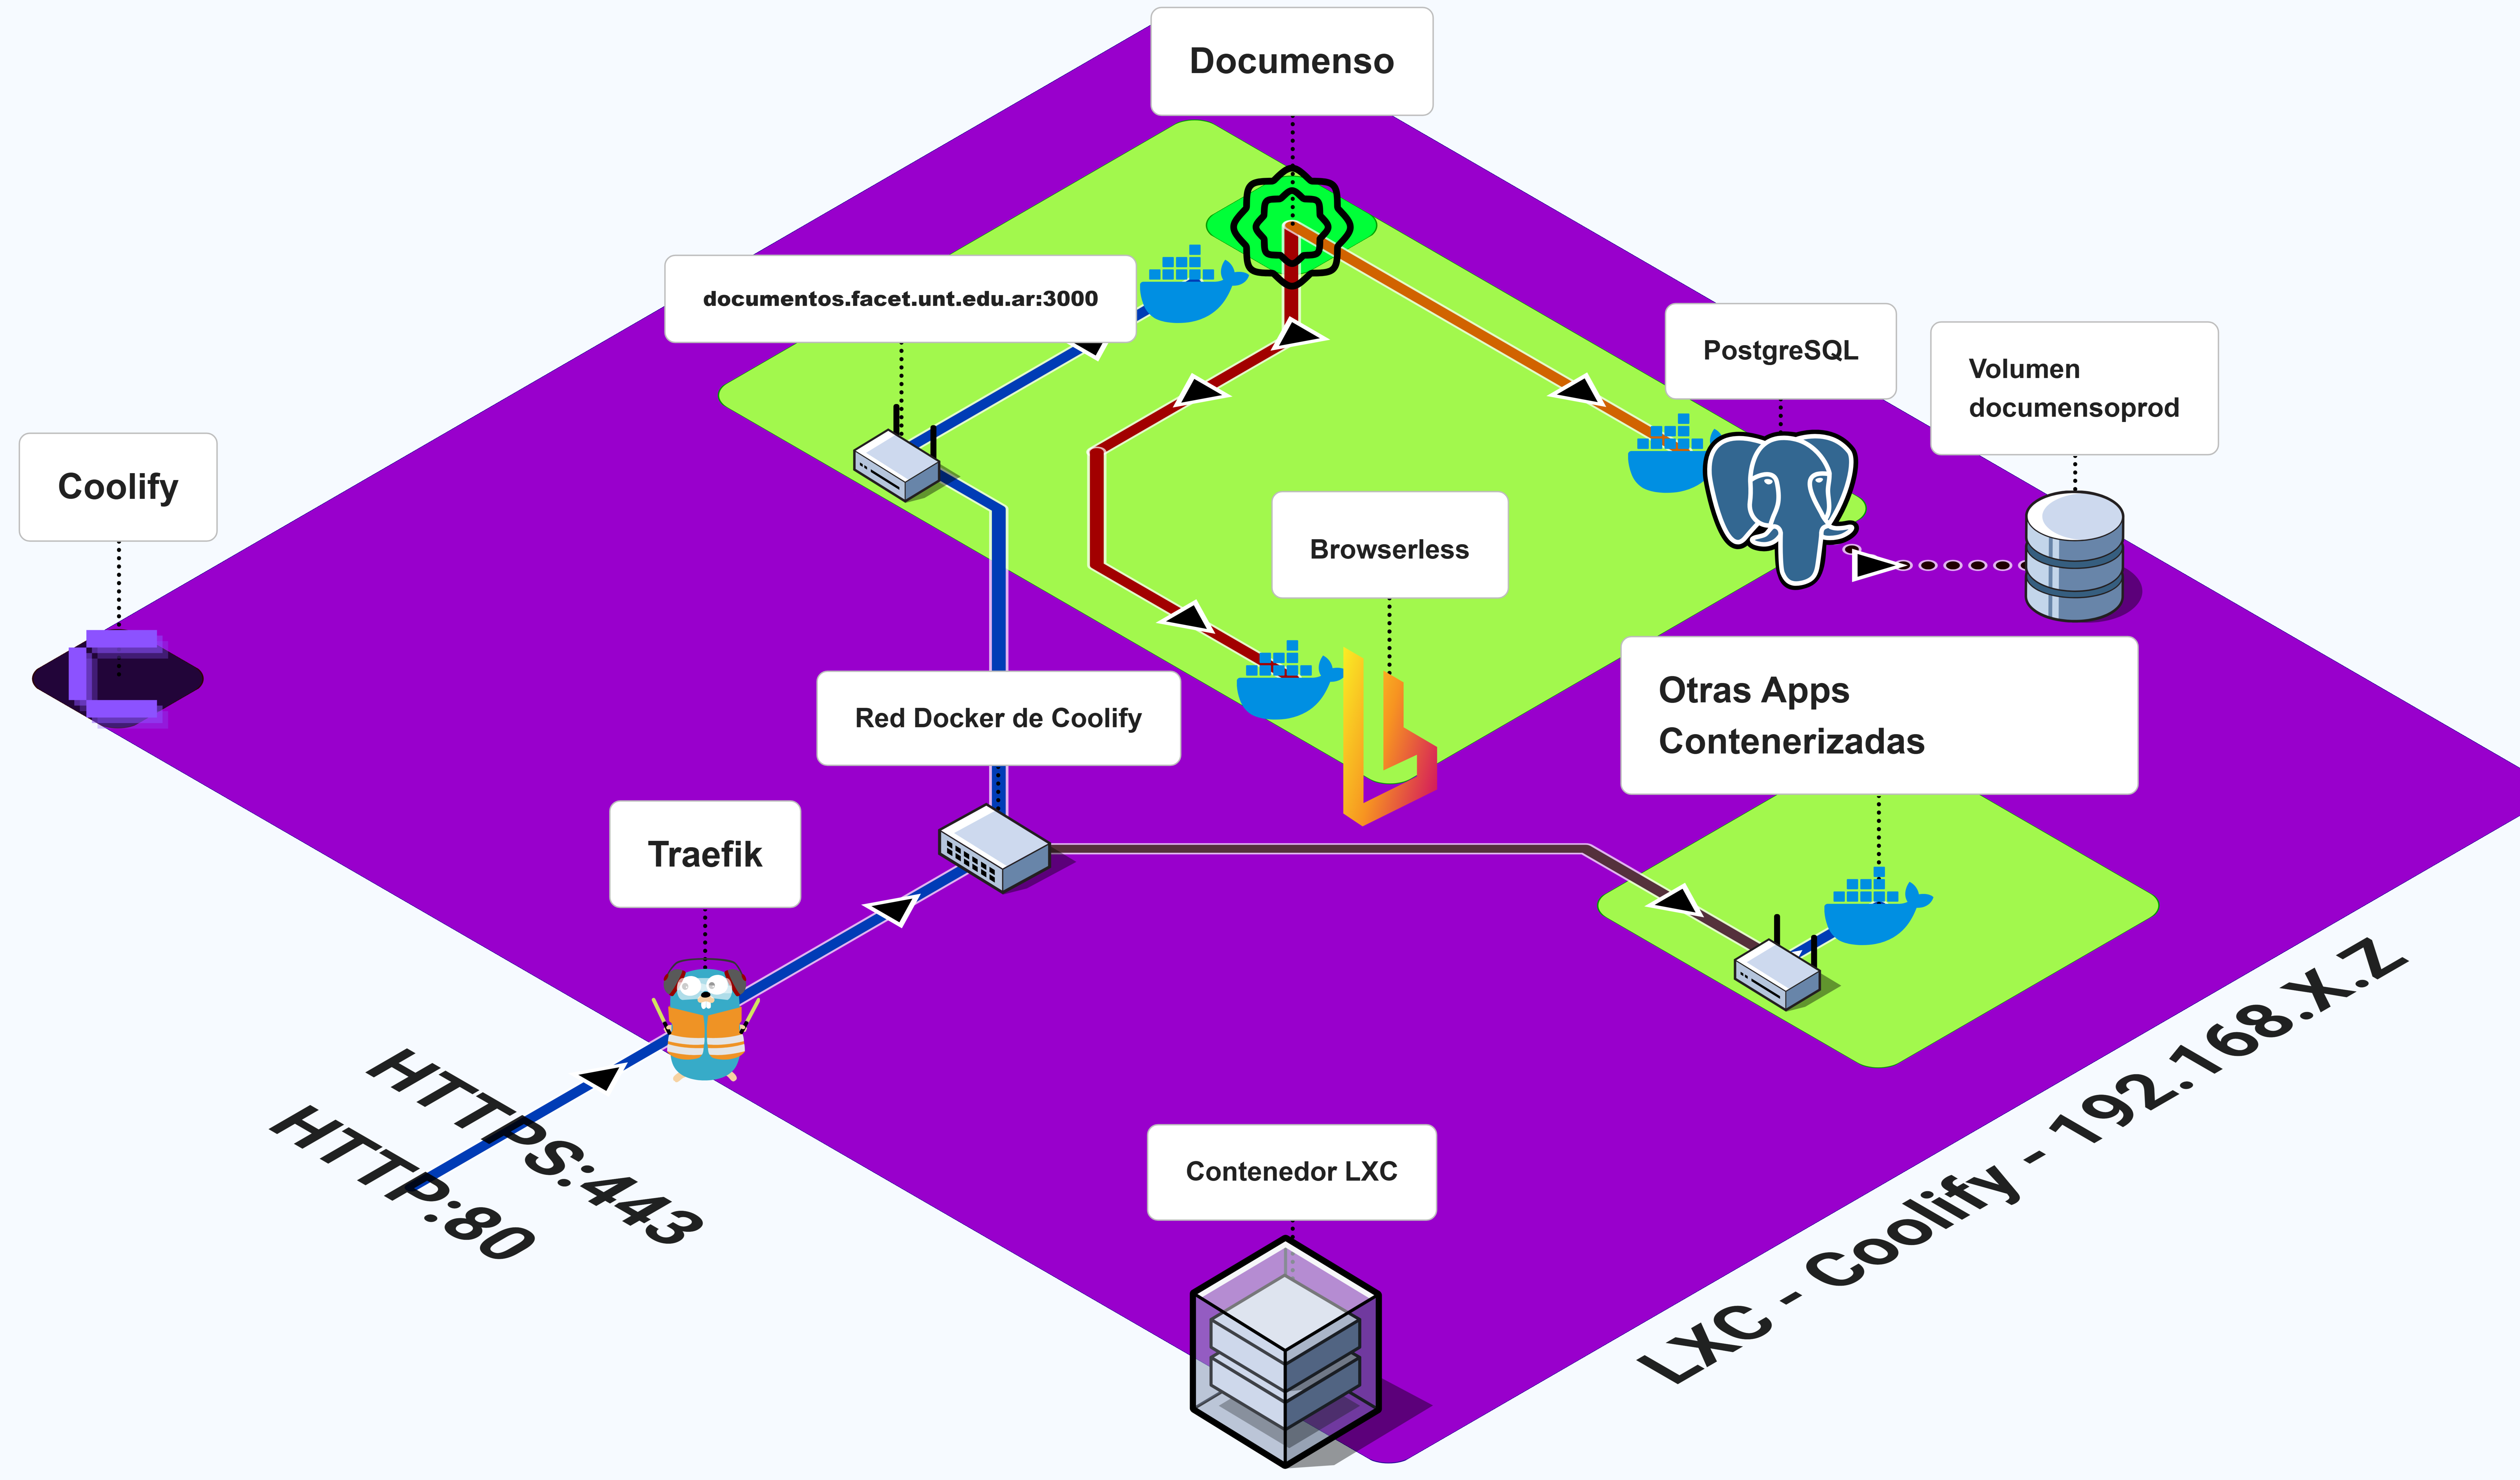
\includegraphics[width=0.9\textwidth]{figuras/capitulo3/3.3.png}
    \caption[Topología interna de la red Docker del despliegue Documenso]{Comunicación entre servicios contenerizados y enrutamiento de Traefik dentro de la red privada del despliegue administrado por Coolify.}
    \label{fig:zoom_seccion_servicios}
\end{figure}


\section{Conectividad con el Almacenamiento de Objetos (Proxy Socat)}
\label{sec:proxy_socat}

La conectividad entre Documenso y MinIO estuvo condicionada por una restricción de diseño de la aplicación: el sistema centraliza la configuración de su almacenamiento S3 a través de una única variable de entorno denominada \texttt{NEXT\_PRIVATE\_UPLOAD\_ENDPOINT}. Al disponer de un único parámetro de configuración, la arquitectura obligó a que tanto el navegador web del usuario (tráfico externo) como el propio servidor interno de la aplicación (tráfico interno) utilizaran una única ruta para acceder al almacenamiento. La solución adoptada fue establecer \nolinkurl{minio.facet.unt.edu.ar} como el dominio público unificado.

Bajo esta configuración, la plataforma opera con dos flujos de datos diferenciados. El primer flujo corresponde a los recursos gráficos de la interfaz, como las imágenes de branding. En este caso, Documenso genera URLs prefirmadas que el navegador consume directamente contra MinIO \cite{documenso_storage_config,documenso_backups}. Si la variable de entorno hubiera contenido una dirección privada de la LAN, como \texttt{192.168.80.24:9000}, este flujo habría fallado porque esa dirección no es enrutable desde Internet y, por lo tanto, no puede ser alcanzada por clientes externos. A esto se suma que las políticas de seguridad del navegador bloquean peticiones desde un origen HTTPS hacia un destino HTTP plano (Mixed Content).

La publicación del dominio \nolinkurl{minio.facet.unt.edu.ar} a través del \textit{reverse proxy} perimetral resolvió este impedimento, pero exigió dos ajustes. Primero, fue necesario configurar el parámetro \texttt{client\_max\_body\_size} en Nginx. Documenso admite cargas de hasta 50~MB por archivo (valor por defecto de la aplicación), por lo que se fijó ese mismo límite para \nolinkurl{documentos.facet.unt.edu.ar}; para \nolinkurl{minio.facet.unt.edu.ar} se estableció 75~MB como margen de seguridad para el peor caso operativo: durante el sellado, la incrustación de firma criptográfica, certificados y metadatos incrementa el tamaño del PDF. De este modo, si un usuario carga un archivo cercano a 50~MB, el sistema conserva holgura suficiente para almacenar la versión firmada sin rechazar la petición. Segundo, en el flujo directo del navegador, fue obligatorio autorizar en MinIO el origen institucional \nolinkurl{https://documentos.facet.unt.edu.ar}. Esto permitió satisfacer las políticas CORS (Cross-Origin Resource Sharing) de MinIO para las peticiones iniciadas desde el navegador. La Figura~\ref{fig:socat_evidencia} evidencia esta secuencia.

\begin{figure}[H]
     \centering
     \begin{subfigure}[b]{0.85\textwidth}
         \centering
         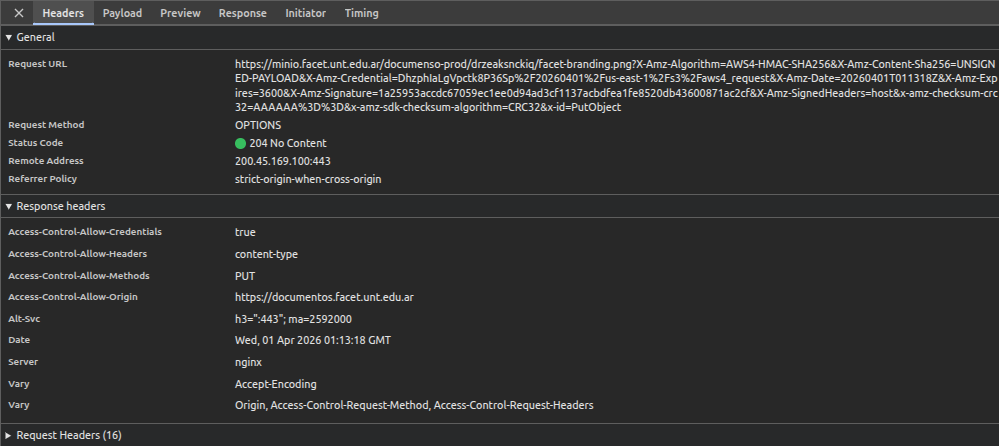
\includegraphics[width=\textwidth]{figuras/capitulo3/requestToMinIO.png}
         \caption{Solicitud preflight OPTIONS del protocolo CORS hacia MinIO.}
         \label{fig:devtools_preflight}
     \end{subfigure}
     \hfill
     \begin{subfigure}[b]{0.85\textwidth}
         \centering
         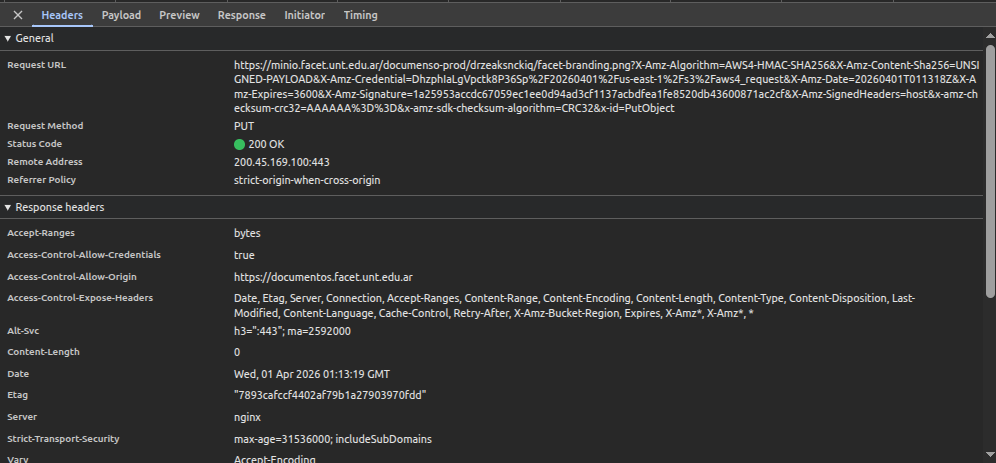
\includegraphics[width=\textwidth]{figuras/capitulo3/requestToMinIO2.png}
         \caption{Petición PUT de carga del recurso gráfico hacia el \textit{bucket} S3.}
         \label{fig:devtools_put}
     \end{subfigure}
        \caption{Evidencia del flujo directo entre la interfaz web de Documenso y MinIO durante la carga de recursos gráficos.}
        \label{fig:socat_evidencia}
\end{figure}

A diferencia del caso anterior, el segundo flujo es indirecto y abarca la carga, descarga y firma de documentos PDF. En este caso, el navegador no interactúa directamente con MinIO, sino que se comunica con la API del servidor interno de Documenso, y es este \textit{backend} quien realiza las operaciones correspondientes sobre el almacenamiento S3.

La Figura~\ref{fig:indirect_flow_devtools} presenta la evidencia de este comportamiento desde la perspectiva del cliente. Durante la descarga de un documento PDF firmado, el navegador emite una petición GET hacia un \textit{endpoint} de la API de la aplicación, en lugar de consumir una URL prefirmada del almacenamiento de objetos. Esto demuestra que el servidor interno actúa como intermediario entre el cliente y MinIO.

\begin{figure}[H]
    \centering
    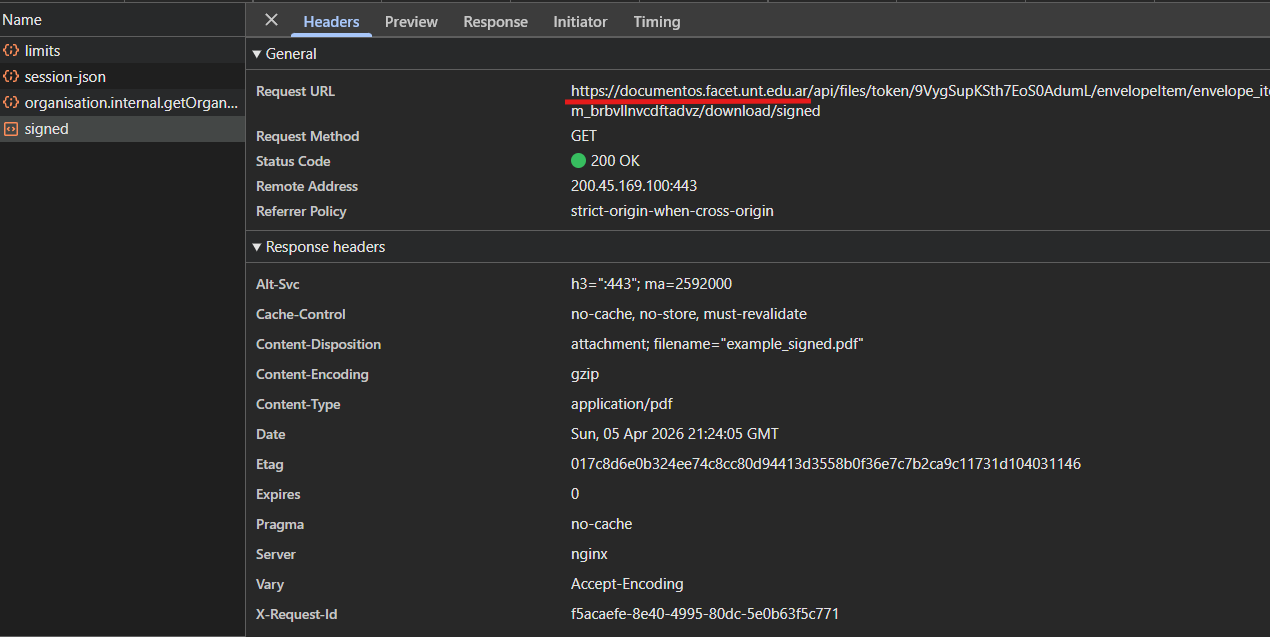
\includegraphics[width=0.88\textwidth]{figuras/capitulo3/http_req_download_pdf_flujo_indirecto.png}
    \caption[Evidencia del flujo indirecto de descarga de PDF firmado]{Descarga indirecta de un documento PDF firmado a través de la API de Documenso.}
    \label{fig:indirect_flow_devtools}
\end{figure}

Para enlazar la red virtual de contenedores con el servidor de almacenamiento TrueNAS, se implementó un contenedor basado en \texttt{socat} dentro de Coolify. El contenedor expone el puerto \texttt{9000} dentro de la red interna de Docker, donde la utilidad queda a la escucha mediante \texttt{TCP4-LISTEN:9000}, y redirige el tráfico TCP hacia la IP del servidor de almacenamiento TrueNAS (\texttt{TCP4:192.168.80.24:9000}). En esta topología, Traefik recibe las peticiones dirigidas a \nolinkurl{minio.facet.unt.edu.ar} y deriva el tráfico entrante hacia ese puerto del contenedor \texttt{socat}, que actúa como puente de red hacia TrueNAS. La composición de este servicio se incluye en el Apéndice~\ref{AppendixB:Compose}. El servicio se desplegó de forma independiente del \textit{stack} principal de Documenso para mantener un túnel reutilizable hacia almacenamiento S3 en futuros proyectos de la facultad.

El diseño final hizo que ambos flujos convergieran en un mismo dominio público, de modo que todo el tráfico dirigido al almacenamiento ---ya se originara externamente en el navegador o fuera reinyectado internamente por el servidor de la aplicación--- atravesara el \textit{reverse proxy} perimetral de la facultad.

La Figura~\ref{fig:flujo_socat_minio} ilustra esta convergencia de los dos flujos hacia el almacenamiento físico. La línea discontinua verde representa el flujo directo originado en el navegador del usuario para las cargas de branding, mientras que la línea discontinua naranja representa el flujo indirecto originado en el \textit{backend} de Documenso para la gestión de documentos PDF. Ambas líneas discontinuas convergen en el \textit{reverse proxy} perimetral Nginx. A partir de ese punto, el tráfico unificado se representa mediante una línea continua rosa que atraviesa Traefik hacia el contenedor \texttt{socat}, y finalmente se transforma en una línea continua azul que enlaza el túnel TCP con el servidor de almacenamiento TrueNAS/MinIO.

\begin{figure}[H]
    \centering
    \includegraphics[width=0.9\textwidth]{figuras/capitulo3/3.4.png}
    \caption[Flujos de acceso a MinIO a través del \textit{proxy} Socat]{Convergencia del flujo directo del navegador y del flujo indirecto del \textit{backend} hacia el servidor de almacenamiento TrueNAS/MinIO a través del \textit{reverse proxy} perimetral, Traefik y el contenedor Socat.}
    \label{fig:flujo_socat_minio}
\end{figure}

\section{Estrategia de Respaldo y Retención de Datos}
\label{sec:estrategia_respaldo_retencion}

La estrategia de preservación de datos se organizó en tres dominios con necesidades de protección diferentes: la base transaccional de PostgreSQL, el repositorio documental almacenado en MinIO y la configuración exportable de la plataforma. Esta separación respondió a un criterio de criticidad operativa: no todos los componentes del sistema se recuperan del mismo modo ni tienen el mismo impacto ante una falla. La base de datos admite respaldos lógicos periódicos, los documentos PDF requieren políticas de retención e inmutabilidad sobre el almacenamiento de objetos, y la reconstrucción del entorno exige conservar las variables de entorno junto con los archivos \texttt{docker-compose.yml} utilizados en producción.

En los tres dominios se aplicó la misma base técnica de almacenamiento S3. La política ILM (Information Lifecycle Management) define el plazo de retención de cada \textit{bucket}, y \textit{Object Lock} en modo \textit{governance} impide modificar o eliminar objetos antes de que venza ese plazo. Para habilitar \textit{Object Lock}, MinIO exige versionado de \textit{buckets}; la operación diaria de la plataforma no depende de ese versionado.

La documentación de Documenso distingue dos alternativas de almacenamiento documental: el almacenamiento en base de datos y el almacenamiento S3 compatible. La Tabla~\ref{tab:documenso_storage_compare} resume las diferencias operativas más relevantes entre ambas, incluida la recomendación explícita de utilizar almacenamiento S3 en despliegues de producción \cite{documenso_storage_config,documenso_backups}.

\begin{table}[!htbp]
    \centering
    \caption[Comparación entre almacenamiento en base de datos y almacenamiento compatible con S3 en Documenso]{Comparación entre las alternativas \texttt{almacenamiento en base de datos} y \texttt{almacenamiento compatible con S3} en Documenso, a partir de la documentación oficial.}
    \label{tab:documenso_storage_compare}
    \begin{tabular}{p{0.24\textwidth} p{0.33\textwidth} p{0.33\textwidth}}
        \toprule
        Aspecto & \texttt{almacenamiento en base de datos} & \texttt{almacenamiento compatible con S3} \\
        \midrule
        Costo de respaldo & Los respaldos de la base crecen junto con el volumen documental. & Requiere respaldar por separado la base y el \textit{bucket} S3. \\
        Rendimiento con archivos grandes & El rendimiento se degrada a medida que aumenta el tamaño del repositorio. & Mantiene un comportamiento más consistente para cargas documentales mayores. \\
        Recomendación de uso & Adecuado para despliegues pequeños o simples. & La documentación lo recomienda para despliegues de producción. \\
        \bottomrule
    \end{tabular}
\end{table}

\subsection{Respaldo lógico de la base de datos PostgreSQL}

En este despliegue, el respaldo lógico de PostgreSQL cubre exclusivamente los datos transaccionales descritos en la Subsección~\ref{subsec:postgresql}. Bajo este criterio, la continuidad operativa no se apoyó exclusivamente en el volumen persistente local del servicio, sino en una política de exportación periódica del contenido de la base hacia un destino independiente, alineada con las estrategias diarias de respaldo automatizado que la documentación de Documenso propone para recuperación a un punto reciente \cite{documenso_backups}. En Coolify se deshabilitó el almacenamiento local de respaldos, los volcados se enviaron al \textit{bucket} \texttt{documenso-backup-databases} en MinIO y se fijó una cuota de 5~GB para ese destino; además, se utilizan marcas de tiempo para garantizar la unicidad de cada respaldo.

El job se programó con la expresión \textit{cron} \texttt{0 3 * * *}, de modo que la exportación se ejecuta diariamente a las 03:00 hacia el destino S3 configurado.

Sobre este \textit{bucket} se aplicó ILM con una retención de 30 días para la versión vigente del respaldo. Esta ventana, junto con la cuota de 5~GB, ofrece un margen operativo prudente para revertir corrupciones o eliminaciones accidentales de la base. Además, se configuró \textit{Object Lock} en modo \textit{governance} por 30 días \cite{minio_object_locking}. Esta frecuencia diaria fija un objetivo práctico de punto de recuperación (\textit{RPO}) de 24 horas para el dominio transaccional. El objetivo de tiempo de recuperación (\textit{RTO}) se mantiene acotado gracias a que Coolify integra importación y restauración directa de volcados desde el almacenamiento S3, lo que reduce la contingencia a una operación asistida desde la interfaz gráfica. El detalle operativo de este procedimiento se documenta en el Apéndice~\ref{AppendixC:RestauracionBD}.

\subsection{Retención e inmutabilidad del repositorio documental}

Los documentos originales cargados por los usuarios y las versiones firmadas se almacenan en el \textit{bucket} \texttt{documenso-prod} del servidor MinIO. Los documentos constituyen el activo \textit{core} del sistema. Como el almacenamiento físico es finito, no pueden conservarse de forma indefinida. Por ello se definió una política ILM de 5 años y, para sostener esa retención, se proyectó y asignó una cuota de 2~TB para el repositorio. El cálculo se apoya en las siguientes restricciones:
\begin{itemize}
    \item Bajo un límite de 300 correos diarios (proveedor SMTP externo) y estimando un promedio de 5 firmantes por trámite ---lo que consume 6 notificaciones por documento (invitaciones y aviso de finalización)---, la plataforma alcanza un techo operativo de 50 trámites por día.
    \item Con un peso promedio estimado de 10~MB por PDF, y considerando que MinIO almacena tanto el archivo original como la versión final firmada (20~MB totales por trámite), el incremento máximo de datos es de 1~GB diario.
    \item Al aplicar la política de retención ILM de 5 años (1825 días), el volumen de datos proyectado es de 1825~GB.
\end{itemize}

En consecuencia, la cuota de 2~TB cubre la demanda máxima teórica proyectada a cinco años, con un margen aproximado del 10\%.

Este límite de 2~TB se estableció considerando la capacidad física del servidor. El volumen de almacenamiento virtual de TrueNAS expone 18,19~TiB al sistema operativo, por lo que la cuota asignada representa aproximadamente el 11\,\% del espacio total.

Sobre esa infraestructura se configuraron en MinIO las políticas de retención del \textit{bucket}. Con el versionado ya habilitado a nivel de plataforma, se aplicó una política ILM de cinco años \cite{minio_ilm_rule_add} y \textit{Object Lock} en modo \textit{governance} por el mismo plazo \cite{minio_object_locking}.

La limitación principal de este dominio de datos aparece en la transición entre ambas capas. La combinación de controles de retención e inmutabilidad protege frente a eliminaciones accidentales, sobrescrituras indebidas y parte de las alteraciones lógicas dentro de MinIO, pero no elimina el punto único de falla representado por el servidor TrueNAS que hospeda el almacenamiento físico. Una falla catastrófica del NAS, una corrupción severa del \textit{pool} o la pérdida total del servidor implicarían la indisponibilidad o pérdida definitiva de los PDF almacenados. Por ello, la replicación o el respaldo \textit{off-site} del repositorio documental hacia un segundo destino S3 compatible se identifica como la mejora de mayor prioridad para una etapa posterior.

\subsection{Resguardo de la configuración del despliegue}

El tercer dominio de protección se orientó a preservar la reconstruibilidad de la plataforma a partir de su configuración exportable. Para ello, se resguardaron las variables de entorno y los archivos \texttt{docker-compose.yml} de cada servicio desplegado, incluida la instancia de Documenso, en el \textit{bucket} \texttt{backups-coolify}. Este resguardo se automatizó mediante un \textit{script} en bash, documentado en el Apéndice~\ref{AppendixB:ConfigBackup}, y ejecutado diariamente con \textit{cron} (\texttt{0 4 * * *}). En lugar de copiar toda la estructura de Coolify, el procedimiento conserva solo los archivos necesarios para reconstruir el entorno. La periodicidad diaria no respondió a cambios frecuentes en la configuración de Documenso, sino a que ese proceso resguarda, de forma unificada, la configuración exportable del conjunto de servicios administrados por Coolify. Sobre dicho \textit{bucket} se definió una cuota de 100~MB y una política ILM con una retención de 180 días para la versión vigente. Al tratarse exclusivamente de archivos de texto plano comprimidos, esta ventana extendida consume un espacio de almacenamiento marginal, pero aporta un valor operativo crítico: garantiza la capacidad de auditar el historial de infraestructura y recuperar configuraciones antiguas (\texttt{.env}) de cualquier proyecto de la facultad ante modificaciones accidentales, eliminaciones o migraciones fallidas.

Este resguardo no sustituye los respaldos de la base de datos ni del repositorio documental, puesto que no conserva ni los datos transaccionales de la aplicación ni los archivos PDF. Su aporte es otro: reduce el tiempo y el esfuerzo requeridos para reconstruir el entorno ante una contingencia severa sobre el servidor. Al preservar la definición de los servicios, las referencias de red y los parámetros de configuración, se evita depender de la reconstrucción manual de secretos, variables y descriptores de despliegue dispersos entre la interfaz de la PaaS y la memoria operativa del administrador.

La guía de mantenimiento de Documenso señala además que, junto con la base de datos y el almacenamiento documental, el certificado de firma y su frase de paso forman parte de los elementos críticos que deben resguardarse \cite{documenso_backups}. En este despliegue, el certificado no se administra como un archivo montado en un volumen, sino como una variable de entorno que contiene el archivo \texttt{.p12} codificado en Base64, junto con la frase de paso inyectada por Coolify. Por ello, el respaldo diario de la configuración también preserva los valores necesarios para restablecer la capacidad de emitir nuevas firmas con la identidad institucional ya configurada.

La estrategia de preservación ofrece puntos de recuperación independientes para el dominio transaccional y para la configuración declarativa del entorno. El riesgo residual ya señalado ---la ausencia de un respaldo externo del repositorio documental--- permanece como la limitación de mayor prioridad para una etapa posterior, dado que una falla física del servidor de almacenamiento dejaría sin recuperación los PDF alojados en MinIO.

\section{Integración del Servicio de Correo Transaccional}

\subsection{Configuración del Servicio de Correo Transaccional (Brevo SMTP)}
\label{subsec:brevo_smtp}

La operación de Documenso requiere un servicio SMTP para emitir invitaciones de firma, recordatorios y notificaciones transaccionales asociadas al avance de cada flujo de firma. Aunque desde el punto de vista técnico hubiera sido posible desplegar un servidor de correo local dentro de la infraestructura institucional, esa alternativa quedó fuera del alcance por su carga operativa. El problema no radica en instalar el servicio, sino en sostener su entregabilidad en producción: reputación de la IP emisora, prevención de bloqueos en listas negras y cumplimiento de políticas de filtrado cada vez más estrictas por parte de proveedores como Gmail u Outlook.

Por ese motivo, el correo saliente se resolvió con Brevo y no con un servidor SMTP propio. La plataforma continuó alojada en la infraestructura de la facultad, pero el envío de notificaciones se delegó a un proveedor externo ya preparado para operar con tasas de entrega adecuadas.

La configuración de Brevo se realizó siguiendo el procedimiento habitual de alta del servicio: creación de la cuenta, verificación del remitente o dominio y obtención de las credenciales SMTP que luego fueron cargadas en Documenso. Durante este trabajo se utilizó el plan gratuito de Brevo, que permite hasta 300 correos diarios. Ese valor se tomó como restricción de dimensionamiento en la estimación presentada en la Sección~\ref{sec:estrategia_respaldo_retencion}. Bajo esa hipótesis, se obtiene un promedio estimado de 50 documentos por día, pero no un límite fijo del sistema, ya que la cantidad real depende del número de firmantes, recordatorios y notificaciones efectivamente enviadas en cada flujo de firma.

Una vez obtenidos en Brevo los registros DNS requeridos para verificar el dominio, se solicitó al área de redes de la facultad su publicación. Se publicaron los registros DNS (TXT) requeridos para la verificación y autorización del dominio.

\subsection{Autenticación Institucional con Google OAuth 2.0}
\label{subsec:google_oauth}

Para el acceso a Documenso se descartó el registro local de usuarios y contraseñas. El motivo principal fue restringir el uso del sistema al personal de la facultad, de modo que ninguna persona ajena pudiera crear una cuenta ni operar la plataforma de firmas. Bajo este criterio, solo los usuarios con cuenta institucional pueden iniciar sesión, cargar documentos y definir los firmantes de cada trámite. Esta restricción alcanza a quienes crean y administran procesos dentro de la plataforma, pero no a los destinatarios de firma: los firmantes pueden pertenecer a cualquier dominio de correo electrónico, ya que el sistema los incorpora como participantes del flujo documental a través de notificaciones transaccionales enviadas por correo.

Se implementó un flujo OAuth 2.0 restringido al ámbito \textit{Interno} de Google Workspace, lo cual garantiza que solo los usuarios del dominio institucional puedan autenticarse.

Para completar la restricción de acceso, se deshabilitó el registro local de nuevas cuentas mediante la configuración correspondiente en las variables de entorno de la aplicación. Con esta medida, el único mecanismo de ingreso quedó limitado a la autenticación mediante Google. El detalle de las variables utilizadas se documenta en el Apéndice~\ref{AppendixB:GoogleOAuth}.

\begin{figure}[!htbp] 
    \centering
    \begin{subfigure}[t]{0.38\textwidth}
        \centering
        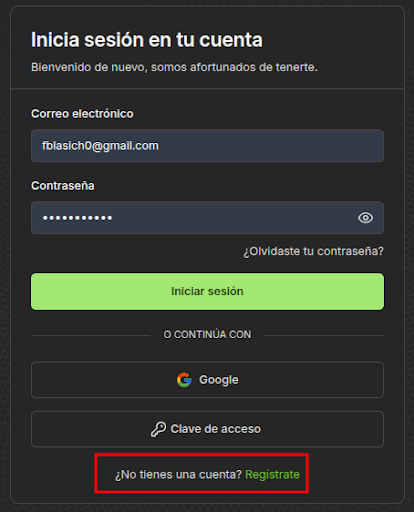
\includegraphics[width=\textwidth]{figuras/capitulo3/login_signup_enabled.png}
        \caption{Pantalla de acceso con registro local habilitado.}
        \label{fig:login_signup_enabled}
    \end{subfigure}
    \hfill
    \begin{subfigure}[t]{0.38\textwidth}
        \centering
        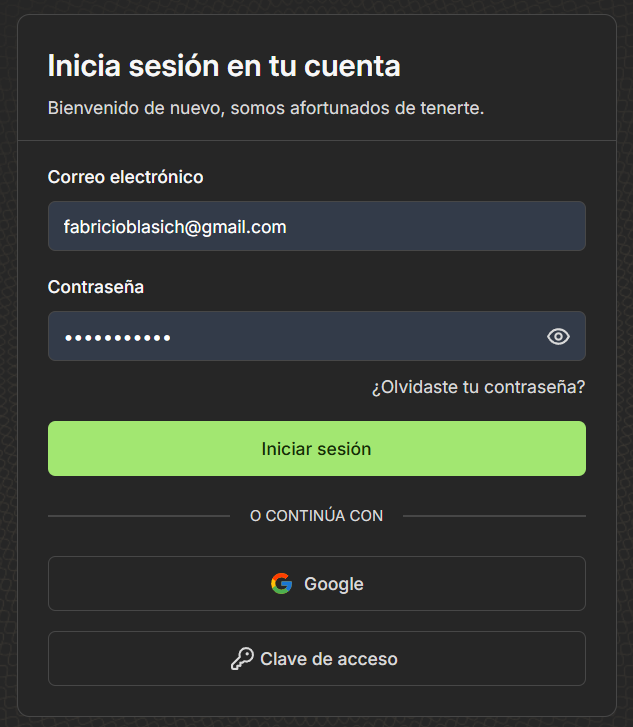
\includegraphics[width=\textwidth]{figuras/capitulo3/login_signup_disabled.png}
        \caption{Pantalla de acceso con registro local deshabilitado.}
        \label{fig:login_signup_disabled}
    \end{subfigure}
    \caption[Restricción del registro local en Documenso]{Comparación de la interfaz de acceso de Documenso con el registro local habilitado y deshabilitado. La eliminación del enlace de registro evidencia que el ingreso al sistema queda limitado a cuentas institucionales.}
    \label{fig:google_oauth_disable_signup}
\end{figure}

La Figura~\ref{fig:google_oauth_disable_signup} muestra el cambio visible en la interfaz de acceso. Con el registro local habilitado aparece el enlace ``\textquestiondown No tienes una cuenta? Reg\'istrate''; al deshabilitarlo, ese enlace desaparece y el ingreso queda limitado a cuentas institucionales.
